\subsection{Objetivo 5 --- avaliação experimental nas bases}

\textit{Avaliar o comportamento dos níveis de Oracle em bases públicas de
classificação.}

Foram usadas $29$ bases públicas (UCI, KEEL e as sintéticas clássicas da literatura
de MCS: P2, Banana, Lithuanian), com $178$ a $19\,020$ amostras, $2$ a $8$ classes e
razão de desbalanceamento de $1.0$ a $71.5$.

\paragraph{Ressalva explícita.} O objetivo 5 menciona preferência por \emph{bases de
imagens} públicas. O catálogo atual privilegia comparabilidade direta com a
literatura de referência (as $28$ bases de Monteiro et al., 2022, mais Magic) em vez
de bases de imagens. É um desvio consciente do enunciado, registrado aqui e nas
pendências do \texttt{ROADMAP}; incorporar bases de imagens é trabalho futuro
imediato, e não altera nenhum dos mecanismos identificados, que dependem da geometria
da fronteira e não do domínio.

\begin{figure}[htbp]
\centering
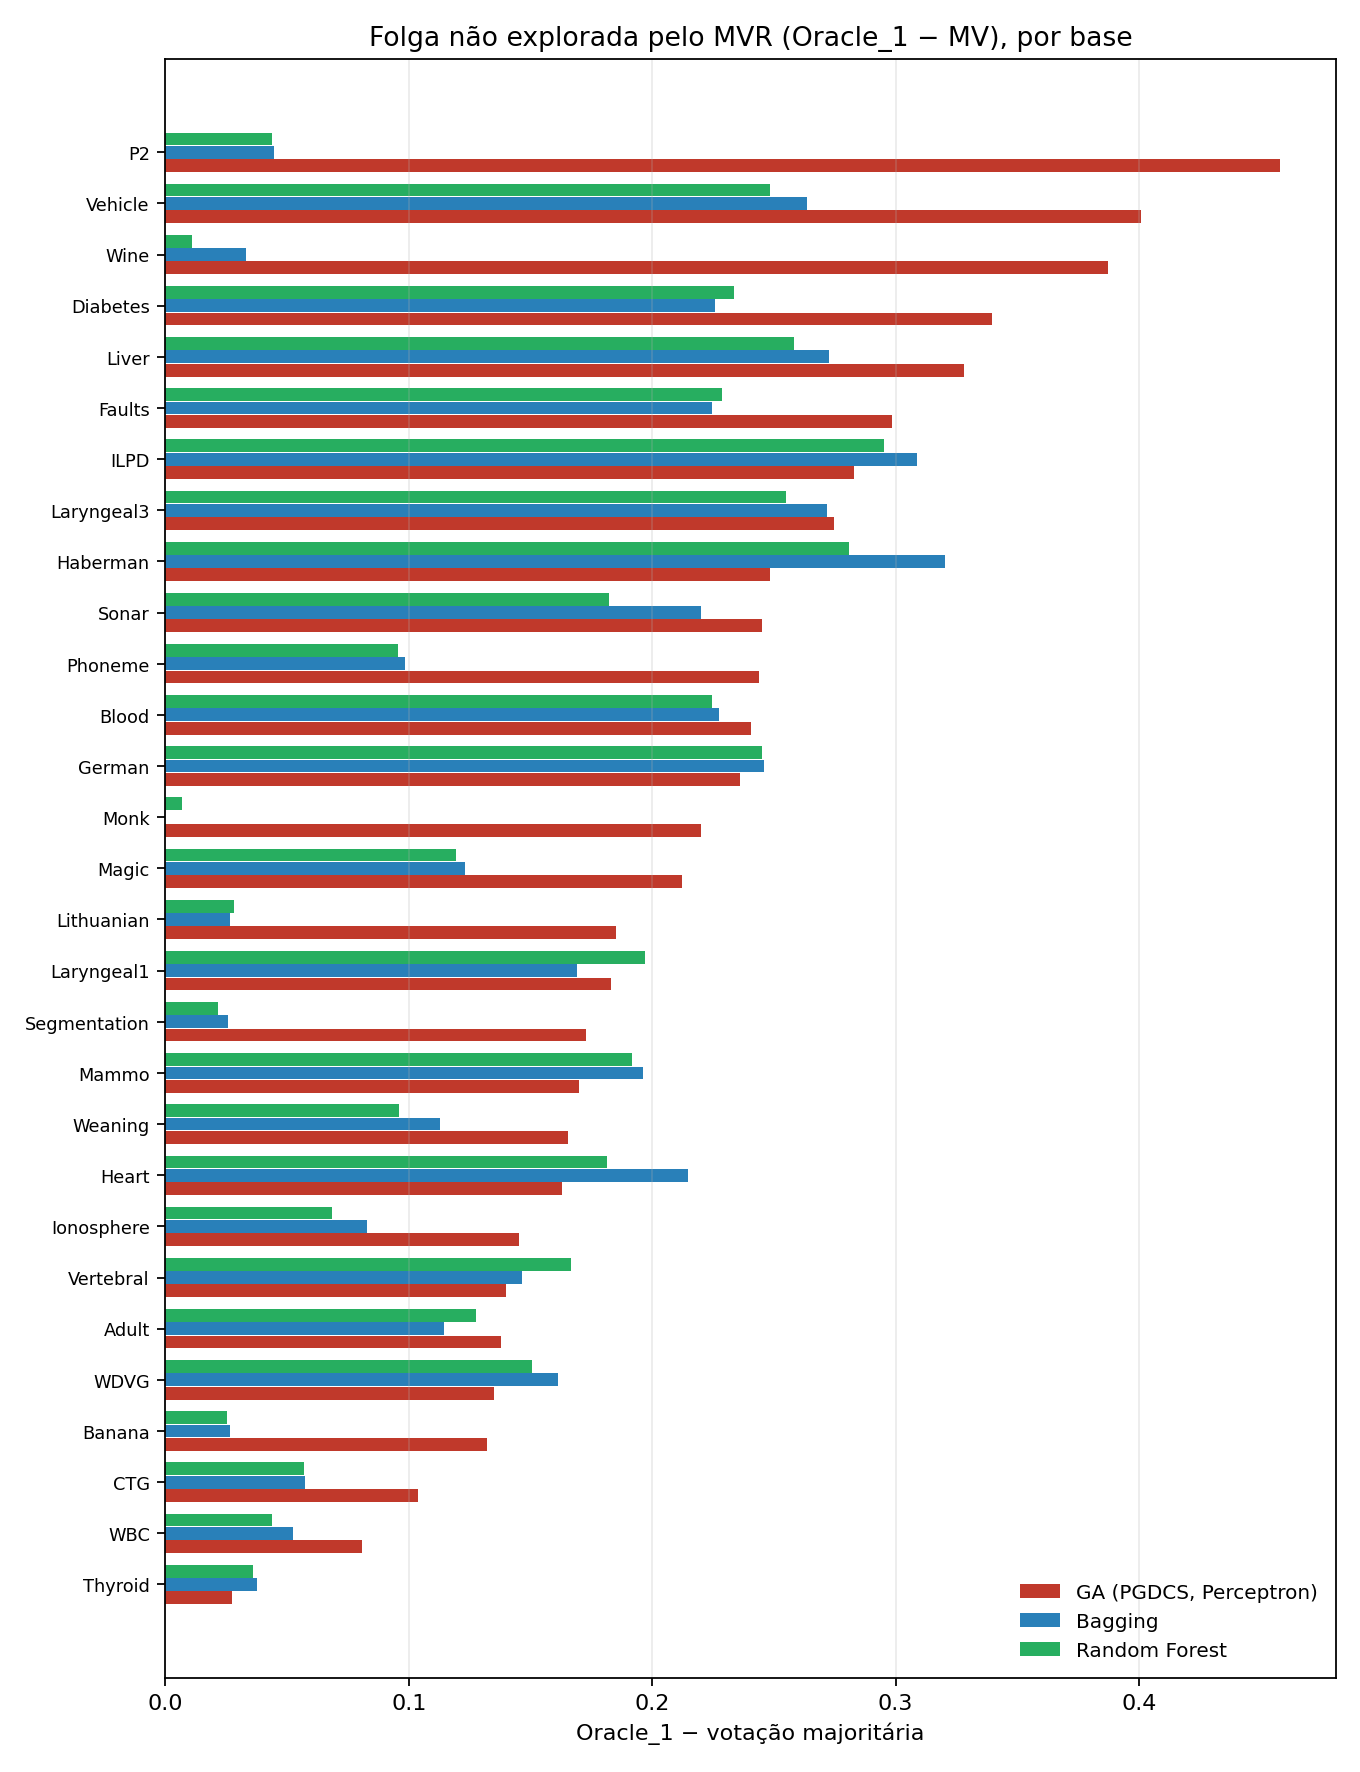
\includegraphics[width=0.92\textwidth]{figuras/fig4_gap_per_dataset.png}
\caption{Folga $\On{1}-\mvr$ por base. A dispersão entre bases ($0.017$ a $0.458$) é
muito maior que a dispersão entre modos ($0.142$ a $0.219$): o potencial não
explorado é sobretudo uma propriedade do problema, não da estratégia de geração.}
\end{figure}
